% Options for packages loaded elsewhere
\PassOptionsToPackage{unicode}{hyperref}
\PassOptionsToPackage{hyphens}{url}
\PassOptionsToPackage{dvipsnames,svgnames,x11names}{xcolor}
%
\documentclass[
]{agujournal2019}

\usepackage{amsmath,amssymb}
\usepackage{iftex}
\ifPDFTeX
  \usepackage[T1]{fontenc}
  \usepackage[utf8]{inputenc}
  \usepackage{textcomp} % provide euro and other symbols
\else % if luatex or xetex
  \usepackage{unicode-math}
  \defaultfontfeatures{Scale=MatchLowercase}
  \defaultfontfeatures[\rmfamily]{Ligatures=TeX,Scale=1}
\fi
\usepackage{lmodern}
\ifPDFTeX\else  
    % xetex/luatex font selection
\fi
% Use upquote if available, for straight quotes in verbatim environments
\IfFileExists{upquote.sty}{\usepackage{upquote}}{}
\IfFileExists{microtype.sty}{% use microtype if available
  \usepackage[]{microtype}
  \UseMicrotypeSet[protrusion]{basicmath} % disable protrusion for tt fonts
}{}
\makeatletter
\@ifundefined{KOMAClassName}{% if non-KOMA class
  \IfFileExists{parskip.sty}{%
    \usepackage{parskip}
  }{% else
    \setlength{\parindent}{0pt}
    \setlength{\parskip}{6pt plus 2pt minus 1pt}}
}{% if KOMA class
  \KOMAoptions{parskip=half}}
\makeatother
\usepackage{xcolor}
\setlength{\emergencystretch}{3em} % prevent overfull lines
\setcounter{secnumdepth}{-\maxdimen} % remove section numbering
% Make \paragraph and \subparagraph free-standing
\makeatletter
\ifx\paragraph\undefined\else
  \let\oldparagraph\paragraph
  \renewcommand{\paragraph}{
    \@ifstar
      \xxxParagraphStar
      \xxxParagraphNoStar
  }
  \newcommand{\xxxParagraphStar}[1]{\oldparagraph*{#1}\mbox{}}
  \newcommand{\xxxParagraphNoStar}[1]{\oldparagraph{#1}\mbox{}}
\fi
\ifx\subparagraph\undefined\else
  \let\oldsubparagraph\subparagraph
  \renewcommand{\subparagraph}{
    \@ifstar
      \xxxSubParagraphStar
      \xxxSubParagraphNoStar
  }
  \newcommand{\xxxSubParagraphStar}[1]{\oldsubparagraph*{#1}\mbox{}}
  \newcommand{\xxxSubParagraphNoStar}[1]{\oldsubparagraph{#1}\mbox{}}
\fi
\makeatother


\providecommand{\tightlist}{%
  \setlength{\itemsep}{0pt}\setlength{\parskip}{0pt}}\usepackage{longtable,booktabs,array}
\usepackage{calc} % for calculating minipage widths
% Correct order of tables after \paragraph or \subparagraph
\usepackage{etoolbox}
\makeatletter
\patchcmd\longtable{\par}{\if@noskipsec\mbox{}\fi\par}{}{}
\makeatother
% Allow footnotes in longtable head/foot
\IfFileExists{footnotehyper.sty}{\usepackage{footnotehyper}}{\usepackage{footnote}}
\makesavenoteenv{longtable}
\usepackage{graphicx}
\makeatletter
\def\maxwidth{\ifdim\Gin@nat@width>\linewidth\linewidth\else\Gin@nat@width\fi}
\def\maxheight{\ifdim\Gin@nat@height>\textheight\textheight\else\Gin@nat@height\fi}
\makeatother
% Scale images if necessary, so that they will not overflow the page
% margins by default, and it is still possible to overwrite the defaults
% using explicit options in \includegraphics[width, height, ...]{}
\setkeys{Gin}{width=\maxwidth,height=\maxheight,keepaspectratio}
% Set default figure placement to htbp
\makeatletter
\def\fps@figure{htbp}
\makeatother
% definitions for citeproc citations
\NewDocumentCommand\citeproctext{}{}
\NewDocumentCommand\citeproc{mm}{%
  \begingroup\def\citeproctext{#2}\cite{#1}\endgroup}
\makeatletter
 % allow citations to break across lines
 \let\@cite@ofmt\@firstofone
 % avoid brackets around text for \cite:
 \def\@biblabel#1{}
 \def\@cite#1#2{{#1\if@tempswa , #2\fi}}
\makeatother
\newlength{\cslhangindent}
\setlength{\cslhangindent}{1.5em}
\newlength{\csllabelwidth}
\setlength{\csllabelwidth}{3em}
\newenvironment{CSLReferences}[2] % #1 hanging-indent, #2 entry-spacing
 {\begin{list}{}{%
  \setlength{\itemindent}{0pt}
  \setlength{\leftmargin}{0pt}
  \setlength{\parsep}{0pt}
  % turn on hanging indent if param 1 is 1
  \ifodd #1
   \setlength{\leftmargin}{\cslhangindent}
   \setlength{\itemindent}{-1\cslhangindent}
  \fi
  % set entry spacing
  \setlength{\itemsep}{#2\baselineskip}}}
 {\end{list}}
\usepackage{calc}
\newcommand{\CSLBlock}[1]{\hfill\break\parbox[t]{\linewidth}{\strut\ignorespaces#1\strut}}
\newcommand{\CSLLeftMargin}[1]{\parbox[t]{\csllabelwidth}{\strut#1\strut}}
\newcommand{\CSLRightInline}[1]{\parbox[t]{\linewidth - \csllabelwidth}{\strut#1\strut}}
\newcommand{\CSLIndent}[1]{\hspace{\cslhangindent}#1}

\usepackage{booktabs}
\usepackage{longtable}
\usepackage{array}
\usepackage{multirow}
\usepackage{wrapfig}
\usepackage{float}
\usepackage{colortbl}
\usepackage{pdflscape}
\usepackage{tabu}
\usepackage{threeparttable}
\usepackage{threeparttablex}
\usepackage[normalem]{ulem}
\usepackage{makecell}
\usepackage{xcolor}
\usepackage{url} %this package should fix any errors with URLs in refs.
\usepackage{lineno}
\usepackage[inline]{trackchanges} %for better track changes. finalnew option will compile document with changes incorporated.
\usepackage{soul}
\linenumbers
\makeatletter
\@ifpackageloaded{caption}{}{\usepackage{caption}}
\AtBeginDocument{%
\ifdefined\contentsname
  \renewcommand*\contentsname{Table of contents}
\else
  \newcommand\contentsname{Table of contents}
\fi
\ifdefined\listfigurename
  \renewcommand*\listfigurename{List of Figures}
\else
  \newcommand\listfigurename{List of Figures}
\fi
\ifdefined\listtablename
  \renewcommand*\listtablename{List of Tables}
\else
  \newcommand\listtablename{List of Tables}
\fi
\ifdefined\figurename
  \renewcommand*\figurename{Figure}
\else
  \newcommand\figurename{Figure}
\fi
\ifdefined\tablename
  \renewcommand*\tablename{Table}
\else
  \newcommand\tablename{Table}
\fi
}
\@ifpackageloaded{float}{}{\usepackage{float}}
\floatstyle{ruled}
\@ifundefined{c@chapter}{\newfloat{codelisting}{h}{lop}}{\newfloat{codelisting}{h}{lop}[chapter]}
\floatname{codelisting}{Listing}
\newcommand*\listoflistings{\listof{codelisting}{List of Listings}}
\makeatother
\makeatletter
\makeatother
\makeatletter
\@ifpackageloaded{caption}{}{\usepackage{caption}}
\@ifpackageloaded{subcaption}{}{\usepackage{subcaption}}
\makeatother
\ifLuaTeX
  \usepackage{selnolig}  % disable illegal ligatures
\fi
\usepackage{bookmark}

\IfFileExists{xurl.sty}{\usepackage{xurl}}{} % add URL line breaks if available
\urlstyle{same} % disable monospaced font for URLs
\hypersetup{
  pdftitle={Lagged Predictions of Next Week Alcohol Use for Precision Mental Health Support},
  pdfauthor={Kendra Wyant; Gaylen E. Fronk; Jiachen Yu; John J. Curtin},
  pdfkeywords={Substance use disorders, Precision mental health},
  colorlinks=true,
  linkcolor={blue},
  filecolor={Maroon},
  citecolor={Blue},
  urlcolor={Blue},
  pdfcreator={LaTeX via pandoc}}


\draftfalse

\begin{document}
\title{Lagged Predictions of Next Week Alcohol Use for Precision Mental
Health Support}

\authors{Kendra Wyant\affil{1}, Gaylen E. Fronk\affil{1}, Jiachen
Yu\affil{1}, John J. Curtin\affil{1}}
\affiliation{1}{Department of Psychology, University of
Wisconsin-Madison, }
\correspondingauthor{John J. Curtin}{jjcurtin@wisc.edu}


\begin{abstract}
We evaluated the performance of a model predicting immediate alcohol
lapses and models with increasing lag time between the prediction time
points and start of the prediction window (24, 72, 168, or 336 hour
lag). Model features were engineered from 4x daily ecological momentary
assessment. Participants (N =151; 51\% male; mean age= 41; 87\% White,
97\% Non-Hispanic) were in early recovery from alcohol use disorder and
provided data for up to three months. We used nested cross-validation to
select and evaluate the best models. Median auROCs were high across
models (range = 0.85 -- 0.89). All lagged models performed significantly
worse than the 0 lag model (probabilities \textgreater{} .95).
Comparisons between adjacent lags revealed significant differences
between 24 and 72 hour lag models and 168 and 336 hour lag models. All
models performed significantly worse for minority groups (not White
vs.~non-Hispanic White, below poverty vs.~above poverty, female
vs.~male).
\end{abstract}




\textsubscript{Source:
\href{https://jjcurtin.github.io/study_lag/index.qmd.html}{Article
Notebook}}

\textsubscript{Source:
\href{https://jjcurtin.github.io/study_lag/index.qmd.html}{Article
Notebook}}

\section{Introduction}\label{introduction}

Precision medicine has been a goal in healthcare for over half a century
(DeRubeis, 2019). Traditionally, precision medicine seeks to answer the
question of \emph{how} we best treat a specific individual, given their
unique combination of genetic, lifestyle, and environmental
characteristics (e.g., which medication is most effective for whom).

Today, this approach is also applied to chronic mental health conditions
(i.e., precision mental health) such as depression, substance use
disorders, and suicide. Mental health conditions are complex,
fluctuating processes. Medical conditions often have clear biological
precursors, which may be treated well with a single medication. In
contrast, mental health conditions are products of numerous psychosocial
factors, and treatments must be selected from a wide array of
psychosocial supports. Moreover, the factors driving mental health
conditions differ between individuals and can change within an
individual over time. Thus, precision mental health must consider both
the \emph{how} and the \emph{when} (e.g., which treatment is most
effective for whom at what moment).

There has been long-standing interest in precision mental health and
substance use disorders. An early example is the Project MATCH research
group, which attempted to match individuals with alcohol use disorder to
their optimal treatment based on baseline measures of individual
characteristics (Project Match Research Group, 1997). Earlier studies,
however, have been constrained to 1) low-dimensional analyses that fail
to capture the complex and heterogeneous nature of substance use
disorders and 2) the use of static distal features to predict a
non-linear, time-varying course of recovery, lapse, and relapse
(Witkiewitz \& Marlatt, 2007).

Recent advances in both machine learning and personal sensing may
address these barriers to successful precision mental health. Machine
learning uses high dimensional inputs that can capture the complexity of
mental health conditions. Moreover, tools from machine learning can be
applied to models to understand which factors are important to a
specific individual at a specific moment in time, addressing the
question of \emph{how}.

Personal sensing allows for frequent, longitudinal measurement of
changes in proximal risk (e.g., for a lapse) with high temporal
precision, for better understanding the \emph{when}. This precision is
particularly important for predicting discrete symptoms or behaviors.
Take the example of lapses, discrete instances of goal inconsistent
substance use. Lapses are a clinically important target for substance
use treatment. They are often an early warning sign of relapse, and
maladaptive responses to lapses can undermine recovery. For some
substances, even a single lapse can result in an overdose and/or death.
It would be unreasonable to expect that we could predict a lapse with
any temporal precision using only features that become more distal as
time progresses. Rather, lapse prediction requires dense, long-term
monitoring of symptoms and related states proximal to the outcome.

Ecological momentary assessment (EMA) may be particularly well-suited
for risk prediction algorithms. It offers momentary subjective insight
into constructs that can be easily mapped onto modular forms of
treatment, such as the relapse prevention model (Marlatt \& Gordon,
1985; Witkiewitz \& Marlatt, 2004). EMA also appears to be well
tolerated by individuals with substance use disorders (Wyant et al.,
2023). Thus, it can serve as an important signal for predicting
substance use outcomes and interpreting clinically relevant features
over a sustained period.

Promising preliminary work suggests it is possible to build EMA models
that predict immediate lapses back to substance use (Bae et al., 2018;
Chih et al., 2014; Soyster et al., 2022; Walters et al., 2021). In a
previous study from our group, we demonstrated that we can do this very
well (Wyant et al., 2024). We used 4X daily EMA with questions designed
to measure theoretically-implicated risk factors including past use,
craving, past pleasant events, past and future risky situations, past
and future stressful events, emotional valence and arousal, and
self-efficacy. We showed that it was possible to predict immediate
alcohol lapses for several different prediction widths with clinically
meaningful accuracy.

Narrow prediction window widths (i.e., next hour or next day) without
any lag time between the prediction time point and start of the
prediction window are well-suited for \emph{Just-in-Time} interventions
that make algorithm-guided recommendations to address immediate risks -
for example, recommending a coping with craving activity when someone
has increased craving, or recommending a guided relaxation video when
someone is reporting recent stressful events. Importantly, these
supports can be available 24/7 (e.g., in a digital therapeutic) for an
individual, allowing them to take action right away.

However, many interventions cannot be self-contained in a digital
therapeutic and take time to set up. For example, someone who has
reported recent past alcohol use and low abstinence self-efficacy might
be encouraged to attend a self-help meeting, plan an outing with
important people in their life, or schedule an appointment with a
therapist. These multimodal interventions (i.e., combined human and
digital interventions) are not available 24/7. A \emph{time-lagged}
model where prediction windows are shifted further into the future
(i.e., away from the prediction time point) could provide patients with
increased lead time to implement supports that might not be immediately
available to them. In these situations, a wider prediction window width
(i.e, one week) may be preferred. Wider window widths yield higher
proportions of positive labels mitigating issues of an unbalanced
outcome. Additionally, when scheduling real world support, it is
important that the lead up time is adequate and not that the prediction
is necessarily temporally precise.

In this study, we evaluated the performance of a model predicting
immediate next week lapses compared to models using increased lag time
between the prediction time points and the start of the prediction
window. Specifically, we used the same EMA features as our immediate
model and trained new models to predict the probability of a lapse
beginning one day (24 hours), three days (72 hours), one week (168
hours), or two weeks (336 hours) into the future. We evaluated each
lagged model to determine if they perform at clinically implementable
levels and assessed the relative difference in performance as lag time
increased.

Additionally, our group is committed to the responsible and transparent
reporting of model performance. Models that work for only a subset of
people, if implemented, could widen existing treatment disparities.
Therefore we reported our models' performance for three dichotomized
demographic groups with known disparities in access to substance use
treatment - race and ethnicity (not White vs.~non-Hispanic White)
(Kilaru et al., 2020; Pinedo, 2019), income (below poverty vs.~above
poverty) (Olfson et al., 2022), and sex at birth (female vs.~male)
(Greenfield et al., 2007; Kilaru et al., 2020).

\section{Methods}\label{methods}

\subsection{Transparency and Openness}\label{transparency-and-openness}

We adhere to research transparency principles that are crucial for
robust and replicable science. We preregistered our data analytic
strategy. We reported how we determined the sample size, all data
exclusions, all manipulations, and all study measures. We provide a
transparency report in the supplement. Finally, our data, analysis
scripts, annotated results, questionnaires, and other study materials
are publicly available (\url{https://osf.io/xta67/}).

\subsection{Participants}\label{participants}

We recruited participants in early recovery (1-8 weeks of abstinence)
from moderate to severe alcohol use disorder in Madison, Wisconsin, US
for a three month longitudinal study. One hundred fifty one participants
were included in our analyses. We used data from all participants
included in our previous study (see (Wyant et al., 2024) for enrollment
and disposition information). This sample size was determined based on
traditional power analysis methods for logistic regression (Hsieh, 1989)
because comparable approaches for machine learning models have not yet
been validated. Participants were recruited through print and targeted
digital advertisements and partnerships with treatment centers. We
required that participants:

\begin{enumerate}
\def\labelenumi{\arabic{enumi}.}
\tightlist
\item
  were age 18 or older,
\item
  could write and read in English,
\item
  had at least moderate AUD (\textgreater= 4 self-reported DSM-5
  symptoms),
\item
  were abstinent from alcohol for 1-8 weeks, and
\item
  were willing to use a single smartphone (personal or study provided)
  while on study.
\end{enumerate}

We also excluded participants exhibiting severe symptoms of psychosis or
paranoia.

\subsection{Procedure}\label{procedure}

Participants completed five study visits over approximately three
months. After an initial phone screen, participants attended an
in-person screening visit to determine eligibility, complete informed
consent, and collect self-report measures. Eligible, consented
participants returned approximately one week later for an intake visit.
Three additional follow-up visits occurred about every 30 days that
participants remained on study. Participants were expected to complete
four daily EMAs while on study. Other personal sensing data streams
(geolocation, cellular communications, sleep quality, and audio
check-ins) were collected as part of the parent grant's aims (R01
AA024391). Participants could earn up to \$150/month if they completed
all study visits, had 10\% or less missing EMA data and opted in to
provide data for other personal sensing data streams.

\subsection{Measures}\label{measures}

\subsubsection{Ecological Momentary
Assessments}\label{ecological-momentary-assessments}

Participants completed four brief (7-10 questions) EMAs daily. The first
and last EMAs of the day were scheduled within one hour of participants'
typical wake and sleep times. The other two EMAs were scheduled randomly
within the first and second halves of their typical day, with at least
one hour between EMAs. Participants learned how to complete the EMA and
the meaning of each question during their intake visit.

On all EMAs, participants reported dates/times of any unreported past
alcohol use. Next, participants rated the maximum intensity of recent
(i.e., since last EMA) experiences of craving, risky situations,
stressful events, and pleasant events. Finally, participants rated their
current affect on two bipolar scales: valence (Unpleasant/Unhappy to
Pleasant/Happy) and arousal (Calm/Sleepy to Aroused/Alert).

On the first EMA each day, participants also rated the likelihood of
encountering risky situations and stressful events in the next week and
the likelihood that they would drink alcohol in the next week (i.e.,
abstinence self-efficacy).

\subsubsection{Individual
Characteristics}\label{individual-characteristics}

We collected self-report information about demographics (age, sex, race,
ethnicity, education, marital status, employment, and income) and AUD
symptom count to characterize our sample. Demographic information was
also included as features in our models and a subset (sex, race,
ethnicity, and income) used for model fairness analyses.

As part of the aims of the parent project we collected many other trait
and state measures throughout the study. A complete list of all measures
can be found on our study's OSF page.

\subsection{Data Analytic Strategy}\label{data-analytic-strategy}

Data preprocessing, modeling, and Bayesian analyses were done in R using
the tidymodels ecosystem (Goodrich et al., 2023; Kuhn, 2022; Kuhn \&
Wickham, 2020). Models were trained and evaluated using high-throughput
computing resources provided by the University of Wisconsin Center for
High Throughput Computing (Center for High Throughput Computing, 2006).

\subsubsection{Predictions}\label{predictions}

Figure~\ref{fig-methods} shows how we established prediction time
points, windows, and lags. All available data up until, but not
including, the prediction time point was used to generate model
predictions. Prediction time points were updated hourly (Panel A). The
first prediction time point for each participant was 24 hours from
midnight on their study start date. This ensured at least 24 hours of
past EMAs for future lapse prediction at these first time points.
Subsequent predictions time points for each participant repeatedly
rolled hour-by-hour until the end of their study participation.

The prediction window width was one week. Prediction windows rolled
forward hour-by-hour with the prediction time point (Panel B). There
were five possible lag times between the prediction time point and start
of the prediction window. A prediction window either started immediately
after the prediction time point (0 lag) or was lagged by 24, 72, 168, or
336 hours.

Therefore, our models provided hour-by-hour probabilities of an alcohol
lapse in the next week pushed out up to two weeks into the future.

\begin{figure}[H]

\centering{

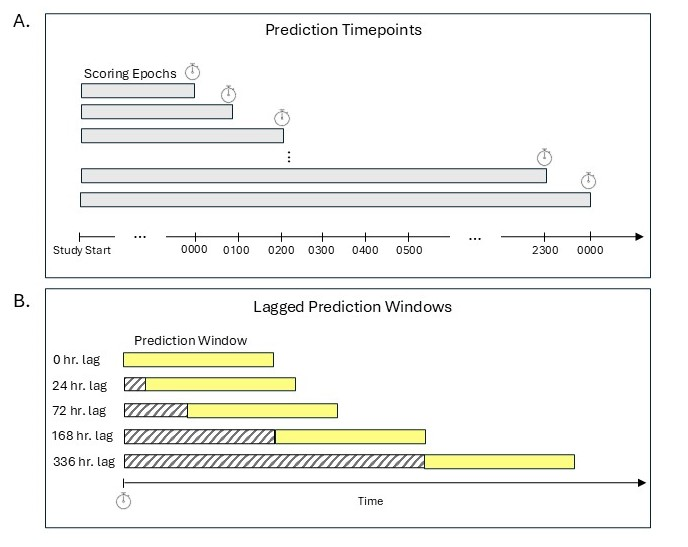
\includegraphics{index_files/figure-latex/notebooks-mak_figures-fig-methods-output-1.jpeg}

}

\caption{\label{fig-methods}We used all available data up until the
prediction timepoint to generate features using varying scoring epochs.
Prediction timepoints rolled forward hour-by-hour (Panel A). Prediction
windows were 1 week wide. A prediction window started immediately after
the prediction timepoint (0 lag) or was lagged by 24, 72, 168, or 336
hours (Panel B).}

\end{figure}%

\textsubscript{Source:
\href{https://jjcurtin.github.io/study_lag/notebooks/mak_figures-preview.html\#cell-fig-methods}{Make
All Figures for Main Manuscript}}

\subsubsection{Labels}\label{labels}

The start and end date/time of past drinking episodes were reported on
the first EMA item. A prediction window was labeled \emph{lapse} if the
start date/hour of any drinking episode fell within that window. A
window was labeled \emph{no lapse} if no alcohol use occurred within
that window +/- 24 hours. If no alcohol use occurred within the window
but did occur within 24 hours of the start or end of the window, the
window was excluded.

We ended up with a total of 270,081 labels for our baseline (no lag)
model, 266,599 labels for our 24 hour lagged model, 259,643 labels for
our 72 hour lagged model, 245,707 labels for our 168 hour lagged model,
and 221,206 labels for our 336 hour lagged model.

\subsubsection{Feature Engineering}\label{feature-engineering}

Features were calculated using only data collected before the start of
each prediction window to ensure our models were making true future
predictions. For our no lag models this included all data prior to the
hour of the start of the prediction window. For our lagged models, the
last EMA data used for feature engineering were collected up to 24
hours, 72 hours, 168 hours, or 336 hours prior to the start of the
prediction window.

A total of 279 features were derived from two data sources:

\begin{enumerate}
\def\labelenumi{\arabic{enumi}.}
\item
  \emph{Demographics}: We created quantitative features for age and
  personal income, and dummy-coded features for sex, race/ethnicity,
  marital status, education, and employment.
\item
  \emph{Previous EMA responses}: We created raw EMA and change features
  for varying scoring epochs (i.e., 12, 24, 48, 72, and 168 hours)
  before the start of the prediction window for all EMA items. Raw
  features included min, max, and median scores for each EMA item across
  all EMAs in each epoch for that participant. We calculated change
  features by subtracting the participants' overall mean score for each
  EMA item (using all EMAs collected before the start of the prediction
  window) from the associated raw feature. We also created raw and
  change features based on the most recent response for each EMA
  question and raw and change rate features from previously reported
  lapses and number of completed EMAs.
\end{enumerate}

Other generic feature engineering steps included imputing missing data
(median imputation for numeric features, mode imputation for nominal
features) and removing zero and near-zero variance features as
determined from held-in data (see Cross-validation section below).

\subsubsection{Model Training and
Evaluation}\label{model-training-and-evaluation}

\paragraph{Model Configurations}\label{model-configurations}

We trained and evaluated five separate classification models: one
baseline (no lag) model and one model for 24 hour, 72 hour, 168 hour,
and 336 hour lagged predictions. We considered four well-established
statistical algorithms (elastic net, XGBoost, regularized discriminant
analysis, and single layer neural networks) that vary across
characteristics expected to affect model performance (e.g., flexibility,
complexity, handling higher-order interactions natively) (Kuhn \&
Johnson, 2018).

Candidate model configurations differed across sensible values for key
hyperparameters. They also differed on outcome resampling method (i.e.,
no resampling and up-sampling and down-sampling of the outcome using
majority/no lapse to minority/lapse ratios ranging from 1:1 to 2:1). We
calibrated predicted probabilities using the beta distribution to
support optimal decision-making under variable outcome distributions
(Kull et al., 2017).

\paragraph{Cross-validation}\label{cross-validation}

We used participant-grouped, nested cross-validation for model training,
selection, and evaluation with auROC. auROC indexes the probability that
the model will predict a higher score for a randomly selected positive
case (lapse) relative to a randomly selected negative case (no lapse).
Grouped cross-validation assigns all data from a participant as either
held-in or held-out to avoid bias introduced when predicting a
participant's data from their own data. We used 1 repeat of 10-fold
cross-validation for the inner loops (i.e., \emph{validation} sets) and
3 repeats of 10-fold cross-validation for the outer loop (i.e.,
\emph{test} sets). Best model configurations were selected using median
auROC across the 10 validation sets. Final performance evaluation of
those best model configurations used median auROC across the 30 test
sets.

\paragraph{Bayesian Model}\label{bayesian-model}

We used a Bayesian hierarchical generalized linear model to estimate the
posterior probability distributions and 95\% Bayesian credible intervals
(CIs) from the 30 held-out test sets for our five best models. Following
recommendations from the rstanarm team and others (Gabry \& Goodrich,
2023; RStudio Team, 2020), we used the rstanarm default autoscaled,
weakly informative, data-dependent priors that take into account the
order of magnitude of the variables to provide some regularization to
stabilize computation and avoid over-fitting.\footnote{Priors were set
  as follows: residual standard deviation \textasciitilde{}
  normal(location=0, scale=exp(2)), intercept (after centering
  predictors) \textasciitilde{} normal(location=2.3, scale=1.3), the two
  coefficients for window width contrasts \textasciitilde{} normal
  (location=0, scale=2.69), and covariance \textasciitilde{}
  decov(regularization=1, concentration=1, shape=1, scale=1).} We set
two random intercepts to account for our resampling method: one for the
repeat, and another for the fold nested within repeat. We specified two
sets of contrasts for model comparisons. The first set compared each
lagged model to the baseline model (0 lag vs.~24 hour lag, 0 lag vs.~72
hour lag, 0 lag vs.~168 lag, 0 lag vs.~336 lag). The second set compared
adjacently lagged models (24 hour lag vs.~72 hour lag, 72 hour lag
vs.~168 hour lag, 168 hour lag vs.~336 hour lag). auROCs were
transformed using the logit function and regressed as a function of
model contrast.

From the Bayesian model we obtained the posterior distribution
(transformed back from logit) and Bayeisan CIs for all five models. To
evaluate our models' overall performance we report the median posterior
probability for auROC and Bayesian CIs. This represents our best
estimate for the magnitude of the auROC parameter for each model. If the
confidence intervals do not contain .5 (chance performance), this
suggests our model is capturing signal in the data.

We then conducted Bayesian model comparisons using our two sets of
contrasts - baseline and adjacent lags. For both model comparisons, we
determined the probability that the models' performances differed
systematically from each other. We also report the precise posterior
probability for the difference in auROCs and the 95\% Bayesian CIs. If
there was a probability \textgreater.95 that the more lagged model's
performance was worse, we labeled the model contrast as significant.

\paragraph{Fairness Analyses}\label{fairness-analyses}

We calculated the median posterior probability and 95\% Bayesian CI for
auROC for each model separately by race and ethnicity (not White
vs.~non-Hispanic White), income (below poverty vs.~above poverty), and
sex at birth (female vs.~male). We conducted Bayesian group comparisons
to assess the likelihood that each model performs differently by group.
We report the median difference and range in posterior probabilities
across all models. The median auROC and Bayesian CIs are reported
separately by group and model in the supplement.\footnote{For our
  fairness analyses, we altered our outer loop resampling method from 3
  x 10 cross-validation to 6 x 5 cross-validation. This method still
  gave us 30 held out tests sets, but by splitting the data across fewer
  folds (i.e., 5 vs.~10) we were able to reduce the likelihood of the
  minority group being absent in any single fold.}

\paragraph{Feature Importance}\label{feature-importance}

We calculated Shapley values in log-odds units for binary classification
models from the 30 test sets to provide a description of the importance
of categories of features across our five models (Lundberg \& Lee,
2017). We averaged the three Shapley values for each observation for
each feature (i.e., across the three repeats) to increase their
stability. An inherent property of Shapley values is their additivity,
allowing us to combine features into feature categories. We created
separate feature categories for each of the nine EMA questions, the
rates of past alcohol use and missing surveys, the time of day and day
of the week of the start of the prediction window, and the seven
demographic variables included in the models. We calculated the local
(i.e., for each observation) importance for each category of features by
adding Shapley values across all features in a category, separately for
each observation. We calculated global importance for each feature
category by averaging the absolute value of the Shapley values of all
features in the category across all observations. These local and global
importance scores based on Shapley values allow us to contextualize
relative feature importance for each model.

\section{Results}\label{results}

\subsection{Demographic and Lapse
Characteristics}\label{demographic-and-lapse-characteristics}

There were approximately equal numbers of men (N=77; 51.0\%) and women
(N=74; 49.0\%) who ranged in age from 21 - 72 years old. The sample was
majority White (N=131; 86.8\%) and non-Hispanic (N=147; 97.4\%).
Participants self-reported a median of 9.0 DSM-5 symptoms of AUD
(mean=8.9; SD=1.9; range=4.0-11.0). Most participants (N=84; 55.6\%)
reported one or more lapses during participation. The median number of
lapses per participant while on-study was 1.0 (mean=6.8; SD = 12.0;
range=0.0-75.0). Table~\ref{tbl-demohtml} provides more detail on
demographic and lapse characteristics of the sample.

\begin{longtable}[]{@{}
  >{\raggedright\arraybackslash}p{(\columnwidth - 10\tabcolsep) * \real{0.4574}}
  >{\raggedleft\arraybackslash}p{(\columnwidth - 10\tabcolsep) * \real{0.0638}}
  >{\raggedleft\arraybackslash}p{(\columnwidth - 10\tabcolsep) * \real{0.0745}}
  >{\raggedright\arraybackslash}p{(\columnwidth - 10\tabcolsep) * \real{0.1170}}
  >{\raggedright\arraybackslash}p{(\columnwidth - 10\tabcolsep) * \real{0.1170}}
  >{\raggedright\arraybackslash}p{(\columnwidth - 10\tabcolsep) * \real{0.1489}}@{}}

\caption{\label{tbl-demohtml}Demographic and Lapse Characteristics}

\tabularnewline

\toprule\noalign{}
\begin{minipage}[b]{\linewidth}\raggedright
var
\end{minipage} & \begin{minipage}[b]{\linewidth}\raggedleft
N
\end{minipage} & \begin{minipage}[b]{\linewidth}\raggedleft
\%
\end{minipage} & \begin{minipage}[b]{\linewidth}\raggedright
M
\end{minipage} & \begin{minipage}[b]{\linewidth}\raggedright
SD
\end{minipage} & \begin{minipage}[b]{\linewidth}\raggedright
Range
\end{minipage} \\
\midrule\noalign{}
\endhead
\bottomrule\noalign{}
\endlastfoot
Age & & & 41 & 11.9 & 21-72 \\
Sex & & & & & \\
Female & 74 & 49.0 & & & \\
Male & 77 & 51.0 & & & \\
Race & & & & & \\
American Indian/Alaska Native & 3 & 2.0 & & & \\
Asian & 2 & 1.3 & & & \\
Black/African American & 8 & 5.3 & & & \\
White/Caucasian & 131 & 86.8 & & & \\
Other/Multiracial & 7 & 4.6 & & & \\
Hispanic, Latino, or Spanish origin & & & & & \\
Yes & 4 & 2.6 & & & \\
No & 147 & 97.4 & & & \\
Education & & & & & \\
Less than high school or GED degree & 1 & 0.7 & & & \\
High school or GED & 14 & 9.3 & & & \\
Some college & 41 & 27.2 & & & \\
2-Year degree & 14 & 9.3 & & & \\
College degree & 58 & 38.4 & & & \\
Advanced degree & 23 & 15.2 & & & \\
Employment & & & & & \\
Employed full-time & 72 & 47.7 & & & \\
Employed part-time & 26 & 17.2 & & & \\
Full-time student & 7 & 4.6 & & & \\
Homemaker & 1 & 0.7 & & & \\
Disabled & 7 & 4.6 & & & \\
Retired & 8 & 5.3 & & & \\
Unemployed & 18 & 11.9 & & & \\
Temporarily laid off, sick leave, or maternity leave & 3 & 2.0 & & & \\
Other, not otherwise specified & 9 & 6.0 & & & \\
Personal Income & & & \$34,298 & \$31,807 & \$0-200,000 \\
Marital Status & & & & & \\
Never married & 67 & 44.4 & & & \\
Married & 32 & 21.2 & & & \\
Divorced & 45 & 29.8 & & & \\
Separated & 5 & 3.3 & & & \\
Widowed & 2 & 1.3 & & & \\
DSM-5 AUD Symptom Count & & & 8.9 & 1.9 & 4-11 \\
Reported 1 or More Lapse During Study Period & & & & & \\
Yes & 84 & 55.6 & & & \\
No & 67 & 44.4 & & & \\
Number of reported lapses & & & 6.8 & 12 & 0-75 \\

\end{longtable}

\textsubscript{Source:
\href{https://jjcurtin.github.io/study_lag/notebooks/mak_tables-preview.html\#cell-tbl-demohtml}{Make
All Tables for Main Manuscript}}

\subsection{Model Evaluation}\label{model-evaluation}

The median auROC across the 30 test sets for our baseline model was high
(median=0.893, IQR=0.045), consistent with our previous
study.\footnote{Baseline models in our previous study yielded a median
  auROC of .895. These models inadvertently excluded income and
  employment as features. We reran models to include these features in
  the current study.} Performance across our lagged models was also high
for the 24 hour lag (median=0.882, IQR=0.039), 72 hour lag
(median=0.868, IQR=0.057), 168 hour lag (median=0.860, IQR=0.062), and
336 hour lag (median=0.856, IQR=0.062).

Histograms of the full posterior probability distributions for auROC for
each model are available in the supplement. The median auROCs from these
posterior distributions were 0.893 (baseline), 0.887 (24 hour lag),
0.875 (72 hour lag), 0.871 (168 hour lag), and 0.852 (336 hour lag).
These values represent our best estimates for the magnitude of the auROC
parameter for each model. The 95\% Bayesian CI for the auROCs for these
models were relatively narrow and did not contain 0.5: baseline
{[}0.876-0.908{]}, 24 hour lag {[}0.869-0.903{]}, 72 hour lag
{[}0.855-0.892{]}, 168 hour lag {[}0.850-0.889{]}, 336 hour lag
{[}0.830-0.872{]}. Panel A in Figure~\ref{fig-1} displays these median
auROCs and 95\% Bayesian CIs by model.

\begin{figure}[H]

\centering{


\includegraphics{index_files/figure-latex/notebooks-mak_figures-fig-1-output-1.png}

}

\caption{\label{fig-1}Panel A depicts posterior probability for area
under ROC curve (auROC) and Bayesian credible intervals by model. Dashed
line indicates a model performing at chance. Panel B depicts difference
in auROCs by demographic group}

\end{figure}%

\textsubscript{Source:
\href{https://jjcurtin.github.io/study_lag/notebooks/mak_figures-preview.html\#cell-fig-1}{Make
All Figures for Main Manuscript}}

\subsection{Model Comparisons}\label{model-comparisons}

\subsubsection{Baseline Contrasts}\label{baseline-contrasts}

The median decrease in auROC for the baseline vs.~24 hour lag model was
0.006 (95\% CI={[}0.000-0.012{]}), yielding a significant probability of
0.960 that the lagged model had worse performance. The median decrease
in auROC for the baseline vs.~72 hour model was 0.018 (95\%
CI={[}0.012-0.025{]}), yielding a significant probability of 1.000 that
the lagged model had worse performance. The median decrease in auROC for
the baseline vs.~168 hour lag model was 0.023 (95\%
CI={[}0.016-0.029{]}), yielding a significant probability of 1.000 that
the lagged model had worse performance. The median decrease in auROC for
the baseline vs.~336 hour lag model was 0.041 (95\%
CI={[}0.033-0.049{]}), yielding a significant probability of 1.000 that
the lagged model had worse performance.

\subsubsection{Adjacent Contrasts}\label{adjacent-contrasts}

The median decrease in auROC for the 24 hour vs.~72 hour lag model was
0.012 (95\% CI={[}0.006-0.019{]}), yielding a significant probability of
1.000 that the 72 hour lag model had worse performance than the 24 hour
lag model. The median decrease in auROC for the 72 hour vs.~168 hour lag
model was 0.004 (95\% CI={[}-0.002-0.011{]}), yielding a non-significant
probability of 0.865 that the 168 hour lag model had worse performance
than the 72 hour lag model. The median decrease in auROC for the 168
hour vs.~336 hour lag model was 0.018 (95\% CI={[}0.011-0.025{]}),
yielding a significant probability of 1.000 that the 336 hour lag model
had worse performance than the 168 hour lag model.

\subsection{Fairness Analyses}\label{fairness-analyses-1}

Panel B in Figure~\ref{fig-1} shows the difference in performance of
each model by race (not White; \emph{N} = 20 vs.~Non-Hispanic White;
\emph{N} = 131), sex at birth (female; \emph{N} = 74 vs.~Male; \emph{N}
= 77), and income (below poverty; \emph{N} = 18 vs.~above poverty;
\emph{N} = 133). All group comparisons were significant (probability
\textgreater{} .95) across models. On average there was a median
decrease in auROC of 0.159 (range 0.107-0.179) for participants who were
not White compared to non-Hispanic White participants. On average there
was a median decrease in auROC of 0.080 (range 0.059-0.116) for female
participants compared to male participants. On average there was a
median decrease in auROC of 0.092 (range 0.086-0.133) for participants
below the federal poverty line compared to participants above the
federal poverty line. Table 1 in the supplement shows the median auROC
and credible intervals separately by group and model.

\subsection{Feature Importance}\label{feature-importance-1}

Global importance (mean \textbar Shapley value\textbar) for feature
categories for each model appears in Panel A of Figure~\ref{fig-shap}.
The top three feature categories for all models were past use, future
efficacy, and craving. Future risky situations were also globally
important across models. This category was ranked as the 4th most
important feature across lagged models (24, 72, 168, and 336 hours). For
the immediate model (0 hour lag), past risky situations were ranked as
the 4th most important feature category and future risky situations was
ranked as the fifth most important. Income was the only demographic
feature that emerged as having high global importance for lapse
prediction (in top 6 for all models). A table of feature categories
ranked by global importance for each model is available in the
supplement.

Panel B shows the local feature importance scores colored by high or low
feature value for the baseline (0 lag) model. Local feature importance
plots for our other models can be found in the supplement. Future
abstinence efficacy, future risky situations, and income appear to have
a linear relationship to lapse prediction. Higher efficacy, fewer future
risky situations, and higher income were associated with a lower
likelihood that the model would predict a lapse. In the supplement, we
plot the relationship between Shapley value and feature score
individually for our overall top five features by model.

\begin{figure}[H]

\centering{


\includegraphics{index_files/figure-latex/notebooks-mak_figures-fig-shap-output-1.png}

}

\caption{\label{fig-shap}Panel A depicts the global importance (mean
\textbar Shapley value\textbar) for feature categories for each model.
Feature categories are ordered by their aggregate global importance
(i.e., total bar length) across the five models. The importance of each
feature category for specific models is displayed separately by color.
Panel B shows the local feature importance for the 0 hour lagged model.}

\end{figure}%

\textsubscript{Source:
\href{https://jjcurtin.github.io/study_lag/notebooks/mak_figures-preview.html\#cell-fig-shap}{Make
All Figures for Main Manuscript}}

\subsection{Discussion}\label{discussion}

\subsubsection{Model Performance}\label{model-performance}

Performance across models was clinically meaningful even up to two weeks
out. Our models yielded median posterior probabilities for auROCs of
0.893 (baseline), 0.887 (24 hour lag), 0.875 (72 hour lag), 0.871 (168
hour lag), and 0.852 (336 hour lag). Our rigorous resampling methods
(grouped, nested, k-fold cross-validation) make us confident that these
are valid estimates of how our models would perform with new
individuals.

Nevertheless, model performance did significantly decrease as models
predicted further into the future. This is unsurprising given what we
know about prediction and substance use. For one, as lag time increases
features become less proximal to the prediction time point. Many
important relapse risk factors are fluctuating processes that can change
day-by-day (if not more frequently). For example, cravings can come on
quickly (e.g., after encountering a person or place that reminds them of
their use) and typically only last for up to 30 minutes. It may be less
important, however, that we miss some of these more fluctuating risk
factors if we consider lagged models as a supplement to immediate lapse
prediction models (i.e., no lag). Lagged prediction models are most
useful for their ability to provide individuals with advanced notice
that they may be at risk for lapsing. This can be used for implementing
more time-intensive recovery supports, such as attending a support
group. On the other hand, an immediate lapse prediction model (i.e., no
lag) is well-suited for detecting and recommending an activity for
immediate risk (e.g., an urge surfing activity for addressing frequent
and recent cravings). Thus, lag time can be customized and layered based
on the intended purpose.

Second, participants only provided EMA for up to three months. Therefore
a lag time of two weeks between the prediction time point and start of
the prediction window prohibits us from using 1/8th of the EMA data for
predictions. In a separate NIH protocol underway, participants are
providing EMA and other sensed data for up to 12 months (Moshontz et
al., 2021). We will better be able to evaluate whether this loss of data
impacted model performance and if we can sustain similar performance
with even longer lags in these data. Still, we wish to emphasize that
our lowest auROC (.85) is still excellent and the benefit of advanced
notice likely outweighs the cost to performance.

We saw mixed evidence that feature importance might change depending on
lag. Past use and craving were the top two features for all models. This
suggests that although these features can change quickly, they are
important enough to consistently emerge as top predictors regardless of
lag time. Recent past risky situations, however, ranked high for the
immediate prediction models, but future anticipated risky situations was
relatively more important for the lagged models.

\subsubsection{Model Fairness}\label{model-fairness}

All models performed worse for women, for people who were not white, and
for people who had an income below the poverty line. The largest
contributing factor is likely the lack of diversity in our training
data. For example, even with our coarse combination of race/ethnicity
(i.e., not White vs.~non-Hispanic White) the minority race/ethnicity
group was largely underrepresented. The best solution to this limitation
would be to recruit a more representative sample. However, there may be
additional methodological considerations for mitigating these issues in
the current data. We could explore upsampling minority group
representation in the data (e.g., using synthetic minority oversampling
technique). We also could adjust the penalty weights so that prediction
errors for minority groups are weighted more heavily than prediction
errors for majority groups.

Lastly, we could consider building models for a specific individual
(i.e., idiographic) (Fisher et al., 2019; Wright \& Zimmermann, 2019).
Unfortunately, a person-specific lapse prediction model would require a
sufficient number of positive labels (i.e., lapses) for that individual.
Waiting until an individual has lapsed multiple (perhaps many) times to
offer help is in direct opposition with our goals. One potential
solution to this conundrum may involve departing from traditional
machine learning algorithms. For example, state space models, which are
grounded in traditional repeated measures designs, inherently capture
time series data and allow for the modeling of how an individual's risk
evolves over time from observable and latent states.

However, we did have equal representation of men and women and we still
saw differences in performance. This difference is likely due to another
source of bias - measurement bias. We chose our EMA items based on
domain expertise and years of relapse risk research. It is possible that
these constructs more precisely describe relapse risk factors for men
than for women. This could mean that more research is needed to identify
relapse risk factors for women. Additionally, data driven (bottom-up)
approaches to creating features could be one way to remove some of the
bias in domain driven (top-down) approaches. For example, using natural
language processing on text message content could allow for new
categories of features to emerge.

\subsubsection{Additional Limitations and Future
Directions}\label{additional-limitations-and-future-directions}

All of the proposed suggestions above for improving model fairness are
current directions in our lab. To increase the diversity of our data, we
recruited a nationally representative sample of people with opioid use
disorder (data collection is near complete) (Moshontz et al., 2021). In
our current sample of participants we are building models that
prioritize accuracy for underrepresented groups. We are also building
models that use sensing methods, like geolocation and text message
content, separately and in conjunction with EMA. In these combined
models we plan to assess whether the relative top features differs by
group. For example, it is possible that data driven features (e.g., from
geolocation) emerge as more important for groups that have been
historically underrepresented in the research on relapse risk factors
driving our self-report measures.

Measurement burden of EMA is also a concern. Research suggests people
can comply with effortful sensing methods (e.g., 4 x daily EMA) while
using substances (Jones et al., 2019; Wyant et al., 2023). However, it
is likely that frequent daily surveys will eventually become too
burdensome when considering long-term monitoring. We plan to build
models that use only 1 x daily EMA to contrast model performance
vs.~assessment burden. We also plan to build models that combine EMA and
passive sensing methods, likes geolocation and evaluate the retained
important features. It is possible that adding other low burden sensing
methods could allow us to reduce the frequency (e.g., 1 x weekly EMA)
and/or length (e.g, 2-3 items) of our EMAs.

Finally, due to prevalent substance use treatment initiation and outcome
disparities among underrepresented groups, it is important to solicit
and consider individual preferences and perceptions of the sensing data
used to build an algorithm-guided risk monitoring support system from
the beginning (i.e., before an intervention is developed). Providing a
support tool only acceptable to a majority group, could widen existing
disparities. In this light we are currently using a mixed-methods design
to assess issues related to feasibility and acceptability by sensing
method and demographic characteristics in our national sample of
participants with opioid use disorder.

This study suggests it is possible to predict alcohol lapses up to two
weeks into the future. This advanced notice could allow patients to
implement multimodal support options not immediately available.
Important steps are still needed to make these models clinically
implementable. Most notably, is the increased fairness in model
performance. However, we remain optimistic as we have already begun to
take several steps in addressing these barriers.

\subsection{References}\label{references}

\phantomsection\label{refs}
\begin{CSLReferences}{1}{0}
\vspace{1em}

\bibitem[\citeproctext]{ref-baeMobilePhoneSensors2018}
Bae, S., Chung, T., Ferreira, D., Dey, A. K., \& Suffoletto, B. (2018).
Mobile phone sensors and supervised machine learning to identify alcohol
use events in young adults: {Implications} for just-in-time adaptive
interventions. \emph{Addictive Behaviors}, \emph{83}, 42--47.
\url{https://doi.org/10.1016/j.addbeh.2017.11.039}

\bibitem[\citeproctext]{ref-chtc}
Center for High Throughput Computing. (2006). Center for high throughput
computing. Center for High Throughput Computing.
\url{https://doi.org/10.21231/GNT1-HW21}

\bibitem[\citeproctext]{ref-chihPredictiveModelingAddiction2014}
Chih, M.-Y., Patton, T., McTavish, F. M., Isham, A. J., Judkins-Fisher,
C. L., Atwood, A. K., \& Gustafson, D. H. (2014). Predictive modeling of
addiction lapses in a mobile health application. \emph{Journal of
Substance Abuse Treatment}, \emph{46}(1), 29--35.
\url{https://doi.org/10.1016/j.jsat.2013.08.004}

\bibitem[\citeproctext]{ref-derubeisHistoryCurrentStatus2019}
DeRubeis, R. J. (2019). The history, current status, and possible future
of precision mental health. \emph{Behaviour Research and Therapy},
\emph{123}, 103506. \url{https://doi.org/10.1016/j.brat.2019.103506}

\bibitem[\citeproctext]{ref-fisherOpenTrialPersonalized2019}
Fisher, A. J., Bosley, H. G., Fernandez, K. C., Reeves, J. W., Soyster,
P. D., Diamond, A. E., \& Barkin, J. (2019). Open trial of a
personalized modular treatment for mood and anxiety. \emph{Behaviour
Research and Therapy}, \emph{116}, 69--79.
\url{https://doi.org/10.1016/j.brat.2019.01.010}

\bibitem[\citeproctext]{ref-gabryPriorDistributionsRstanarm2023}
Gabry, J., \& Goodrich, B. (2023). Prior {Distributions} for rstanarm
{Models}. \emph{CRAN R-Project}.
https://cran.r-project.org/web/packages/rstanarm/vignettes/priors.html.

\bibitem[\citeproctext]{ref-goodrichRstanarmBayesianApplied2023}
Goodrich, B., Gabry, J., Ali, I., \& Brilleman, S. (2023). Rstanarm:
{Bayesian Applied Regression Modeling} via {Stan}.

\bibitem[\citeproctext]{ref-greenfieldSubstanceAbuseTreatment2007}
Greenfield, S. F., Brooks, A. J., Gordon, S. M., Green, C. A., Kropp,
F., McHugh, R. K., et al. (2007). Substance abuse treatment entry,
retention, and outcome in women: {A} review of the literature.
\emph{Drug and Alcohol Dependence}, \emph{86}(1), 1--21.
\url{https://doi.org/10.1016/j.drugalcdep.2006.05.012}

\bibitem[\citeproctext]{ref-hsiehSampleSizeTables1989}
Hsieh, F. (1989). Sample size tables for logistic regression.
\emph{Statistics in Medicine}, \emph{8}, 795--802.

\bibitem[\citeproctext]{ref-jonesComplianceEcologicalMomentary2019a}
Jones, A., Remmerswaal, D., Verveer, I., Robinson, E., Franken, I. H.
A., Wen, C. K. F., \& Field, M. (2019). Compliance with ecological
momentary assessment protocols in substance users: A meta-analysis.
\emph{Addiction (Abingdon, England)}, \emph{114}(4), 609--619.
\url{https://doi.org/gfsjzg}

\bibitem[\citeproctext]{ref-kilaruIncidenceTreatmentOpioid2020}
Kilaru, A. S., Xiong, A., Lowenstein, M., Meisel, Z. F., Perrone, J.,
Khatri, U., et al. (2020). Incidence of {Treatment} for {Opioid Use
Disorder Following Nonfatal Overdose} in {Commercially Insured
Patients}. \emph{JAMA Network Open}, \emph{3}(5), e205852.
\url{https://doi.org/10.1001/jamanetworkopen.2020.5852}

\bibitem[\citeproctext]{ref-kuhnTidyposteriorBayesianAnalysis2022}
Kuhn, M. (2022). Tidyposterior: {Bayesian Analysis} to {Compare Models}
using {Resampling Statistics}.

\bibitem[\citeproctext]{ref-kuhnAppliedPredictiveModeling2018}
Kuhn, M., \& Johnson, K. (2018). \emph{Applied {Predictive Modeling}}
(1st ed. 2013, Corr. 2nd printing 2018 edition). New York: Springer.
\url{https://doi.org/10.1007/978-1-4614-6849-3}

\bibitem[\citeproctext]{ref-kuhnTidymodelsCollectionPackages2020}
Kuhn, M., \& Wickham, H. (2020). Tidymodels: A collection of packages
for modeling and machine learning using tidyverse principles.

\bibitem[\citeproctext]{ref-kullSigmoidsHowObtain2017}
Kull, M., Filho, T. M. S., \& Flach, P. (2017). Beyond sigmoids: {How}
to obtain well-calibrated probabilities from binary classifiers with
beta calibration. \emph{Electronic Journal of Statistics}, \emph{11}(2),
5052--5080. \url{https://doi.org/10.1214/17-EJS1338SI}

\bibitem[\citeproctext]{ref-lundbergUnifiedApproachInterpreting2017}
Lundberg, S. M., \& Lee, S.-I. (2017). A unified approach to
interpreting model predictions. In \emph{Proceedings of the 31st
{International Conference} on {Neural Information Processing Systems}}
(pp. 4768--4777). Red Hook, NY, USA: Curran Associates Inc.

\bibitem[\citeproctext]{ref-marlattRelapsePreventionMaintenance1985}
Marlatt, G. A., \& Gordon, J. R. (Eds.). (1985). \emph{Relapse
{Prevention}: {Maintenance Strategies} in the {Treatment} of {Addictive
Behaviors}} (First edition). New York: The Guilford Press.

\bibitem[\citeproctext]{ref-moshontzProspectivePredictionLapses2021}
Moshontz, H., Colmenares, A. J., Fronk, G. E., Sant'Ana, S. J., Wyant,
K., Wanta, S. E., et al. (2021). Prospective {Prediction} of {Lapses} in
{Opioid Use Disorder}: {Protocol} for a {Personal Sensing Study}.
\emph{JMIR Research Protocols}, \emph{10}(12), e29563.
\url{https://doi.org/10.2196/29563}

\bibitem[\citeproctext]{ref-olfsonHealthcareCoverageService2022}
Olfson, M., Mauro, C., Wall, M. M., Choi, C. J., Barry, C. L., \&
Mojtabai, R. (2022). Healthcare coverage and service access for
low-income adults with substance use disorders. \emph{Journal of
Substance Abuse Treatment}, \emph{137}, 108710.
\url{https://doi.org/10.1016/j.jsat.2021.108710}

\bibitem[\citeproctext]{ref-pinedoCurrentReexaminationRacial2019}
Pinedo, M. (2019). A current re-examination of racial/ethnic disparities
in the use of substance abuse treatment: {Do} disparities persist?
\emph{Drug and Alcohol Dependence}, \emph{202}, 162--167.
\url{https://doi.org/10.1016/j.drugalcdep.2019.05.017}

\bibitem[\citeproctext]{ref-projectmatchresearchgroupMatchingAlcoholismTreatments1997}
Project Match Research Group, U. S. (1997). Matching alcoholism
treatments to client heterogeneity: {Project MATCH Posttreatment}
drinking outcomes. \emph{Journal of Studies on Alcohol}, \emph{58}(1),
7--29.

\bibitem[\citeproctext]{ref-rstudioteamRStudioIntegratedDevelopment2020}
RStudio Team. (2020). {RStudio}: {Integrated Development} for {R}.
Boston, MA: RStudio, Inc.

\bibitem[\citeproctext]{ref-soysterPooledPersonspecificMachine2022}
Soyster, P. D., Ashlock, L., \& Fisher, A. J. (2022). Pooled and
person-specific machine learning models for predicting future alcohol
consumption, craving, and wanting to drink: {A} demonstration of
parallel utility. \emph{Psychology of Addictive Behaviors: Journal of
the Society of Psychologists in Addictive Behaviors}, \emph{36}(3),
296--306. \url{https://doi.org/10.1037/adb0000666}

\bibitem[\citeproctext]{ref-waltersUsingMachineLearning2021}
Walters, S. T., Businelle, M. S., Suchting, R., Li, X., Hébert, E. T.,
\& Mun, E.-Y. (2021). Using machine learning to identify predictors of
imminent drinking and create tailored messages for at-risk drinkers
experiencing homelessness. \emph{Journal of Substance Abuse Treatment},
\emph{127}, 108417. \url{https://doi.org/10.1016/j.jsat.2021.108417}

\bibitem[\citeproctext]{ref-witkiewitzRelapsePreventionAlcohol2004}
Witkiewitz, K., \& Marlatt, G. A. (2004). Relapse prevention for alcohol
and drug problems: {That} was zen, this is tao. \emph{American
Psychologist}, \emph{59}(4), 224--235.
\url{https://doi.org/10.1037/0003-066X.59.4.224}

\bibitem[\citeproctext]{ref-witkiewitzModelingComplexityPosttreatment2007}
Witkiewitz, K., \& Marlatt, G. A. (2007). Modeling the complexity of
post-treatment drinking: {It}'s a rocky road to relapse. \emph{Clinical
Psychology Review}, \emph{27}(6), 724--738.
\url{https://doi.org/10.1016/j.cpr.2007.01.002}

\bibitem[\citeproctext]{ref-wrightAppliedAmbulatoryAssessment2019}
Wright, A. G. C., \& Zimmermann, J. (2019). Applied {Ambulatory
Assessment}: {Integrating Idiographic} and {Nomothetic Principles} of
{Measurement}. \emph{Psychological Assessment}, \emph{31}(12),
1467--1480. \url{https://doi.org/10.1037/pas0000685}

\bibitem[\citeproctext]{ref-wyantAcceptabilityPersonalSensing2023}
Wyant, K., Moshontz, H., Ward, S. B., Fronk, G. E., \& Curtin, J. J.
(2023). Acceptability of {Personal Sensing Among People With Alcohol Use
Disorder}: {Observational Study}. \emph{JMIR mHealth and uHealth},
\emph{11}(1), e41833. \url{https://doi.org/10.2196/41833}

\bibitem[\citeproctext]{ref-wyantMachineLearningModels2023}
Wyant, K., Sant'Ana, S. J. K., Fronk, G., \& Curtin, J. J. (2024).
Machine learning models for temporally precise lapse prediction in
alcohol use disorder. \emph{Psychopathology and Clinical Science}.
\url{https://doi.org/10.31234/osf.io/cgsf7}

\end{CSLReferences}



\end{document}
